\documentclass[12pt,a4paper]{article}

% Essential packages
\usepackage[utf8]{inputenc}
\usepackage[T1]{fontenc}
\usepackage{geometry}
\usepackage{graphicx}
\usepackage{amsmath}
\usepackage{amssymb}
\usepackage{booktabs}
\usepackage{array}
\usepackage{longtable}
\usepackage{multirow}
\usepackage{hyperref}
\usepackage{xcolor}
\usepackage{fancyhdr}
\usepackage{titlesec}
\usepackage{tocloft}
\usepackage{listings}
\usepackage{enumitem}
\usepackage{float}
\usepackage{tikz}
\usepackage{pgfgantt}
\usepackage{forest}

% Page setup
\geometry{margin=1in}

% Colors
\definecolor{primarygold}{RGB}{212, 175, 55}
\definecolor{darkbg}{RGB}{26, 26, 26}
\definecolor{textgray}{RGB}{100, 100, 100}
\definecolor{codebg}{RGB}{245, 245, 245}

% Hyperlink setup
\hypersetup{
    colorlinks=true,
    linkcolor=blue!70!black,
    filecolor=magenta,
    urlcolor=cyan!70!black,
    citecolor=green!50!black
}

% Header/Footer
\pagestyle{fancy}
\fancyhf{}
\fancyhead[L]{\textit{JewelQR System - Software Engineering Project}}
\fancyhead[R]{\thepage}
\fancyfoot[C]{\textit{February 2026}}

% Section formatting
\titleformat{\section}{\Large\bfseries\color{blue!70!black}}{\thesection}{1em}{}
\titleformat{\subsection}{\large\bfseries}{\thesubsection}{1em}{}

% Code listing style
\lstset{
    backgroundcolor=\color{codebg},
    basicstyle=\ttfamily\small,
    breaklines=true,
    frame=single,
    numbers=left,
    numberstyle=\tiny\color{gray},
    keywordstyle=\color{blue},
    commentstyle=\color{green!50!black},
    stringstyle=\color{orange}
}

\begin{document}

% ============================================================================
% TITLE PAGE
% ============================================================================
\begin{titlepage}
    \centering
    \vspace*{1cm}
    
    {\Huge\bfseries SOFTWARE ENGINEERING\\[0.3cm]PROJECT SUBMISSION\par}
    
    \vspace{1.5cm}
    
    {\LARGE\bfseries Jewelry QR Composition, Cloud Inventory\\& Dynamic Pricing System\par}
    
    \vspace{0.5cm}
    
    {\large A Web-Based Solution for Jewelry Retail Management\par}
    
    \vspace{2cm}
    
    \begin{tabular}{ll}
        \textbf{Submitted By:} & Bhavya Dhoot \\[0.3cm]
        \textbf{Roll Number:} & 23BCE0007 \\[0.3cm]
        \textbf{Branch:} & Computer Science and Engineering (B.Tech III Year) \\[0.3cm]
        \textbf{Semester:} & 6th Semester \\[0.3cm]
        \textbf{Subject:} & Software Engineering \\[0.3cm]
        \textbf{Submitted To:} & Parthiban K \\[0.3cm]
        \textbf{Date:} & 3rd February 2026
    \end{tabular}
    
    \vfill
    
    {\small Document Version: 1.7.0 | Production Ready - Security Hardened\par}
\end{titlepage}

% ============================================================================
% TABLE OF CONTENTS
% ============================================================================
\newpage
\tableofcontents
\newpage

% ============================================================================
% SECTION 1: PROJECT TITLE
% ============================================================================
\section{Project Title}

\textbf{\Large Jewelry QR Composition, Cloud Inventory \& Dynamic Pricing System}

\vspace{0.5cm}

The project aims to build a web-based application that helps jewelry shop owners manage their inventory using QR codes. Each jewelry item gets a unique QR code that stores its composition details like gold weight, purity, and diamond specifications. Customers can scan the QR code to see item details and get real-time pricing based on current gold and diamond rates.

\subsection{Core Features}

\begin{table}[H]
\centering
\begin{tabular}{|p{4cm}|p{10cm}|}
\hline
\textbf{Feature} & \textbf{Description} \\
\hline
Auto-SKU Generation & Unique SKUs with category prefix (e.g., CHN-000017) \\
\hline
QR Code Creation & QR codes contain only SKU - item details fetched from database on scan \\
\hline
Dynamic Pricing & Calculate real-time prices based on current gold/diamond rates \\
\hline
Gold Purity Pricing & Automatic purity factor: 24K=100\%, 22K=92\%, 18K=76\%, 14K=60\% \\
\hline
Dynamic Diamond Categories & Add, edit, toggle active/inactive, delete diamond types via Settings \\
\hline
Labour Cost & Automatic calculation: Labour Rate $\times$ Gold Weight \\
\hline
Role-Based Access & Admin and Staff roles with different permissions \\
\hline
Cloud Storage & MongoDB database for persistent storage \\
\hline
\end{tabular}
\caption{Core System Features}
\end{table}

% ============================================================================
% SECTION 2: ABSTRACT
% ============================================================================
\section{Abstract}

Managing jewelry inventory is a hassle for most small and medium jewelry retailers in India. They still rely on manual calculation of prices and paper-based records, which leads to errors and customer trust issues.

This project solves these problems by creating a QR-based inventory system. Here's how it works:

\begin{itemize}
    \item Shop owners can create entries for each jewelry item with all composition details
    \item The system generates a unique QR code for each item
    \item Customers can scan the QR code using their phone and view item details
    \item They can enter current gold/diamond rates to calculate real-time prices
    \item The system supports different diamond types (Moti, Pear, Markish, Round) and classifications (Real vs CVD)
\end{itemize}

The frontend is built using plain HTML, CSS, and JavaScript - no heavy frameworks needed. QRCode.js library is used for generating QR codes and Html5QrcodeScanner for camera-based scanning.

The main benefit is \textbf{transparency} - customers can verify what they're paying for, and shop owners can maintain accurate records without manual paperwork.

% ============================================================================
% SECTION 3: PROBLEM STATEMENT
% ============================================================================
\section{Problem Statement}

\subsection{Why This Project?}

The following problems were observed in local jewelry shops:

\subsubsection{Price Calculation Errors}
\begin{itemize}
    \item Shop staff calculate prices manually using calculators
    \item Different staff may quote different prices for the same item
    \item Human error leads to disputes
\end{itemize}

\subsubsection{No Transparency}
\begin{itemize}
    \item Customers have no way to verify if the quoted gold weight is correct
    \item Diamond quality claims cannot be verified
    \item Trust issues between buyers and sellers
\end{itemize}

\subsubsection{Inventory Management}
\begin{itemize}
    \item Most shops use register books or Excel sheets
    \item No easy way to search or track items
    \item Difficult to audit stock
\end{itemize}

\subsubsection{Price Fluctuations}
\begin{itemize}
    \item Gold prices change daily
    \item Staff must manually recalculate prices every morning
    \item Old price tags cause confusion
\end{itemize}

\subsubsection{Diamond Classification}
\begin{itemize}
    \item Natural diamonds and CVD (lab-grown) diamonds have different prices
    \item No system to distinguish and price them correctly
    \item Different diamond shapes (Moti, Pear, etc.) need separate tracking
\end{itemize}

\subsection{Our Solution}

A QR-based web application that:
\begin{itemize}
    \item Stores complete item composition in the QR code itself
    \item Allows real-time price calculation with current rates
    \item Works on any smartphone browser
    \item Requires no app installation
    \item Has admin controls for managing inventory and rates
\end{itemize}

% ============================================================================
% SECTION 4: PROJECT SCHEDULING
% ============================================================================
\section{Project Scheduling}

Project scheduling is the process of identifying all activities required to complete a project and arranging them in proper sequence with appropriate time estimates. This section covers the complete scheduling analysis using industry-standard techniques.

\subsection{Tools Used for Project Scheduling}

\begin{table}[H]
\centering
\begin{tabular}{|l|p{6cm}|p{5cm}|}
\hline
\textbf{Tool/Technique} & \textbf{Purpose} & \textbf{Software Used} \\
\hline
Gantt Chart & Visual timeline of project tasks & Microsoft Project / GanttProject \\
\hline
PERT Chart & Probabilistic time estimation & Microsoft Visio / Draw.io \\
\hline
CPM Analysis & Critical path identification & Manual calculation + Excel \\
\hline
WBS & Work breakdown structure & Microsoft Word / MindMap \\
\hline
Resource Allocation & Staff and resource planning & Microsoft Excel \\
\hline
\end{tabular}
\caption{Project Scheduling Tools Used}
\end{table}

\subsection{Activity List and Duration Estimates}

\begin{table}[H]
\centering
\small
\begin{tabular}{|c|p{5.5cm}|c|c|c|}
\hline
\textbf{ID} & \textbf{Activity} & \textbf{Predecessor} & \textbf{Duration (Days)} & \textbf{Resources} \\
\hline
A & Requirements Gathering & - & 5 & 2 \\
\hline
B & Technology Stack Selection & A & 2 & 1 \\
\hline
C & UI/UX Design & A & 7 & 1 \\
\hline
D & Database Schema Design & B & 4 & 1 \\
\hline
E & Backend API Development & D & 12 & 2 \\
\hline
F & Frontend Development & C & 15 & 2 \\
\hline
G & QR Code Integration & E, F & 5 & 1 \\
\hline
H & Authentication System & E & 4 & 1 \\
\hline
I & Dashboard Development & F, H & 6 & 1 \\
\hline
J & Testing \& Debugging & G, I & 7 & 2 \\
\hline
K & Documentation & J & 4 & 1 \\
\hline
L & Deployment & K & 3 & 1 \\
\hline
\end{tabular}
\caption{Activity List with Duration and Dependencies}
\end{table}

\subsection{Gantt Chart}

The Gantt Chart provides a visual timeline representation of the project schedule, showing task durations and their overlaps.

\begin{figure}[H]
\centering
\resizebox{\textwidth}{!}{%
\begin{ganttchart}[
    hgrid,
    vgrid={*6{draw=gray!30}, *1{draw=gray!60}},
    x unit=0.35cm,
    y unit chart=0.5cm,
    title height=1,
    bar height=0.5,
    group height=0.3,
    bar/.append style={fill=blue!40},
    group/.append style={fill=blue!20},
    milestone/.append style={fill=red!60},
    title label font=\scriptsize,
    bar label font=\tiny,
    group label font=\tiny\bfseries
]{1}{49}
    \gantttitle{Project Timeline (Weeks)}{49} \\
    \gantttitle{W1}{7} \gantttitle{W2}{7} \gantttitle{W3}{7} \gantttitle{W4}{7} \gantttitle{W5}{7} \gantttitle{W6}{7} \gantttitle{W7}{7} \\
    
    \ganttgroup{Phase 1: Planning}{1}{7} \\
    \ganttbar{A: Requirements}{1}{5} \\
    \ganttbar{B: Tech Stack}{6}{7} \\
    
    \ganttgroup{Phase 2: Design}{6}{12} \\
    \ganttbar{C: UI/UX Design}{6}{12} \\
    \ganttbar{D: DB Schema}{8}{11} \\
    
    \ganttgroup{Phase 3: Development}{12}{33} \\
    \ganttbar{E: Backend API}{12}{23} \\
    \ganttbar{F: Frontend}{13}{27} \\
    \ganttbar{G: QR Integration}{28}{32} \\
    \ganttbar{H: Auth System}{24}{27} \\
    \ganttbar{I: Dashboard}{28}{33} \\
    
    \ganttgroup{Phase 4: Testing}{34}{40} \\
    \ganttbar{J: Testing}{34}{40} \\
    
    \ganttgroup{Phase 5: Delivery}{41}{47} \\
    \ganttbar{K: Documentation}{41}{44} \\
    \ganttbar{L: Deployment}{45}{47} \\
    \ganttmilestone{Project Complete}{47}
\end{ganttchart}
}%
\caption{Gantt Chart for JewelQR Project (47 Days / 7 Weeks)}
\end{figure}

\subsection{Activity Network Model (AON - Activity on Node)}

The Activity Network Model shows the logical sequence and dependencies between project activities.

\begin{figure}[H]
\centering
\resizebox{0.95\textwidth}{!}{%
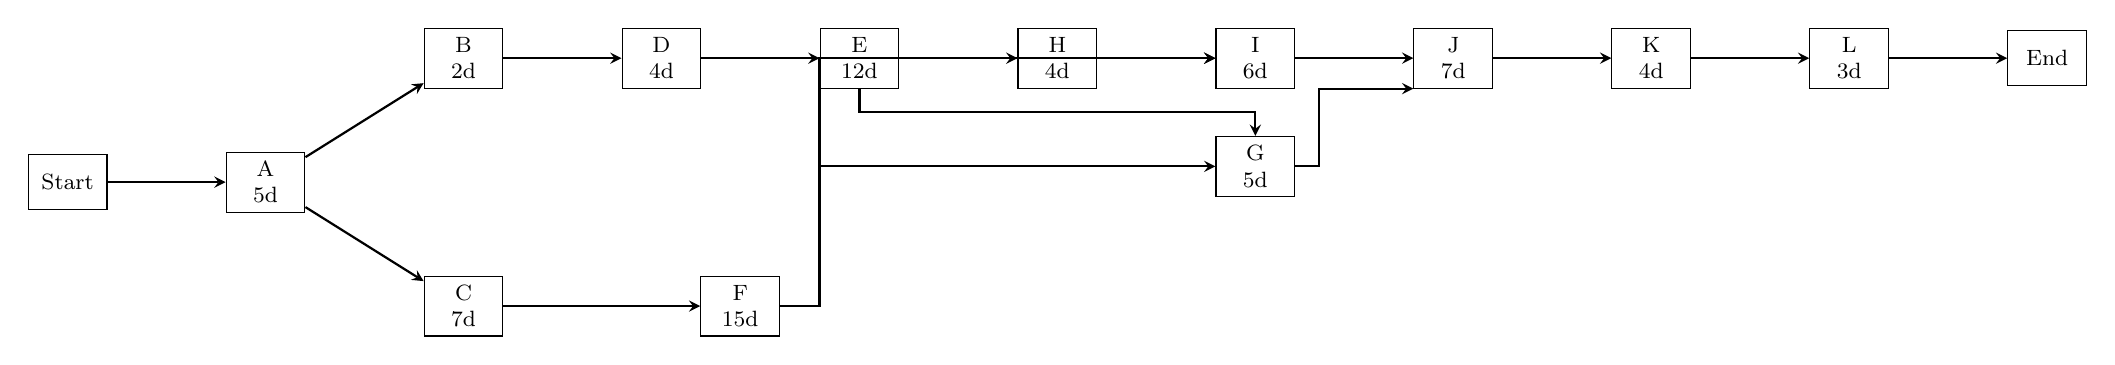
\begin{tikzpicture}[
    node distance=1.8cm and 1.5cm,
    activity/.style={rectangle, draw, minimum width=1cm, minimum height=0.7cm, font=\footnotesize, align=center},
    arrow/.style={->, thick, >=stealth}
]
    % Row 1 (Top path: B -> D -> E -> H)
    \node[activity] (start) {Start};
    \node[activity, right=of start] (A) {A\\5d};
    \node[activity, above right=0.8cm and 1.5cm of A] (B) {B\\2d};
    \node[activity, right=of B] (D) {D\\4d};
    \node[activity, right=of D] (E) {E\\12d};
    \node[activity, right=of E] (H) {H\\4d};
    
    % Row 2 (Bottom path: C -> F)
    \node[activity, below right=0.8cm and 1.5cm of A] (C) {C\\7d};
    \node[activity, right=2.5cm of C] (F) {F\\15d};
    
    % Row 3 (Merge path: G, I -> J -> K -> L -> End)
    \node[activity, right=of H] (I) {I\\6d};
    \node[activity, below=0.6cm of I] (G) {G\\5d};
    \node[activity, right=of I] (J) {J\\7d};
    \node[activity, right=of J] (K) {K\\4d};
    \node[activity, right=of K] (L) {L\\3d};
    \node[activity, right=of L] (end) {End};
    
    % Arrows - Left section
    \draw[arrow] (start) -- (A);
    \draw[arrow] (A) -- (B);
    \draw[arrow] (A) -- (C);
    \draw[arrow] (B) -- (D);
    \draw[arrow] (D) -- (E);
    \draw[arrow] (C) -- (F);
    
    % Arrows - Middle section  
    \draw[arrow] (E) -- (H);
    \draw[arrow] (E.south) -- ++(0,-0.3) -| (G.north);
    \draw[arrow] (F.east) -- ++(0.5,0) |- (G.west);
    \draw[arrow] (F.east) -- ++(0.5,0) |- (I.west);
    \draw[arrow] (H) -- (I);
    
    % Arrows - Right section
    \draw[arrow] (G.east) -- ++(0.3,0) |- (J.south west);
    \draw[arrow] (I) -- (J);
    \draw[arrow] (J) -- (K);
    \draw[arrow] (K) -- (L);
    \draw[arrow] (L) -- (end);
\end{tikzpicture}
}%
\caption{Activity-on-Node (AON) Network Diagram}
\end{figure}

\subsection{PERT Chart Analysis}

PERT (Program Evaluation and Review Technique) uses three time estimates for each activity:
\begin{itemize}
    \item \textbf{Optimistic (O)}: Best-case scenario
    \item \textbf{Most Likely (M)}: Expected duration
    \item \textbf{Pessimistic (P)}: Worst-case scenario
\end{itemize}

\textbf{Expected Time Formula:}
\begin{equation}
T_E = \frac{O + 4M + P}{6}
\end{equation}

\begin{table}[H]
\centering
\small
\begin{tabular}{|c|p{4cm}|c|c|c|c|c|}
\hline
\textbf{ID} & \textbf{Activity} & \textbf{O} & \textbf{M} & \textbf{P} & \textbf{$T_E$} & \textbf{$\sigma^2$} \\
\hline
A & Requirements Gathering & 3 & 5 & 9 & 5.33 & 1.00 \\
\hline
B & Tech Stack Selection & 1 & 2 & 4 & 2.17 & 0.25 \\
\hline
C & UI/UX Design & 5 & 7 & 12 & 7.50 & 1.36 \\
\hline
D & Database Schema Design & 2 & 4 & 7 & 4.17 & 0.69 \\
\hline
E & Backend API Development & 8 & 12 & 20 & 12.67 & 4.00 \\
\hline
F & Frontend Development & 10 & 15 & 25 & 15.83 & 6.25 \\
\hline
G & QR Code Integration & 3 & 5 & 9 & 5.33 & 1.00 \\
\hline
H & Authentication System & 2 & 4 & 7 & 4.17 & 0.69 \\
\hline
I & Dashboard Development & 4 & 6 & 10 & 6.33 & 1.00 \\
\hline
J & Testing \& Debugging & 4 & 7 & 13 & 7.50 & 2.25 \\
\hline
K & Documentation & 2 & 4 & 7 & 4.17 & 0.69 \\
\hline
L & Deployment & 1 & 3 & 6 & 3.17 & 0.69 \\
\hline
\end{tabular}
\caption{PERT Time Estimates (Days)}
\end{table}

\textbf{Variance Formula:}
\begin{equation}
\sigma^2 = \left(\frac{P - O}{6}\right)^2
\end{equation}

\subsection{Critical Path Method (CPM)}

The Critical Path is the longest path through the network, determining the minimum project duration.

\subsubsection{Forward Pass Calculation (Earliest Start/Finish)}

\begin{table}[H]
\centering
\begin{tabular}{|c|c|c|c|c|}
\hline
\textbf{Activity} & \textbf{Duration} & \textbf{ES} & \textbf{EF} & \textbf{Predecessor} \\
\hline
A & 5 & 0 & 5 & - \\
\hline
B & 2 & 5 & 7 & A \\
\hline
C & 7 & 5 & 12 & A \\
\hline
D & 4 & 7 & 11 & B \\
\hline
E & 12 & 11 & 23 & D \\
\hline
F & 15 & 12 & 27 & C \\
\hline
G & 5 & 27 & 32 & E, F \\
\hline
H & 4 & 23 & 27 & E \\
\hline
I & 6 & 27 & 33 & F, H \\
\hline
J & 7 & 33 & 40 & G, I \\
\hline
K & 4 & 40 & 44 & J \\
\hline
L & 3 & 44 & 47 & K \\
\hline
\end{tabular}
\caption{Forward Pass - Earliest Start (ES) and Earliest Finish (EF)}
\end{table}

\subsubsection{Backward Pass Calculation (Latest Start/Finish)}

\begin{table}[H]
\centering
\begin{tabular}{|c|c|c|c|c|c|}
\hline
\textbf{Activity} & \textbf{Duration} & \textbf{LS} & \textbf{LF} & \textbf{Slack} & \textbf{Critical?} \\
\hline
A & 5 & 0 & 5 & 0 & \textbf{Yes} \\
\hline
B & 2 & 5 & 7 & 0 & \textbf{Yes} \\
\hline
C & 7 & 5 & 12 & 0 & \textbf{Yes} \\
\hline
D & 4 & 7 & 11 & 0 & \textbf{Yes} \\
\hline
E & 12 & 11 & 23 & 0 & \textbf{Yes} \\
\hline
F & 15 & 12 & 27 & 0 & \textbf{Yes} \\
\hline
G & 5 & 28 & 33 & 1 & No \\
\hline
H & 4 & 23 & 27 & 0 & \textbf{Yes} \\
\hline
I & 6 & 27 & 33 & 0 & \textbf{Yes} \\
\hline
J & 7 & 33 & 40 & 0 & \textbf{Yes} \\
\hline
K & 4 & 40 & 44 & 0 & \textbf{Yes} \\
\hline
L & 3 & 44 & 47 & 0 & \textbf{Yes} \\
\hline
\end{tabular}
\caption{Backward Pass - Latest Start (LS), Latest Finish (LF), and Slack Time}
\end{table}

\subsubsection{Critical Path Identification}

\textbf{Note:} This project has \textbf{two parallel critical paths} with the same total duration:

\vspace{0.3cm}
\noindent\fbox{\parbox{\textwidth-2\fboxsep-2\fboxrule}{%
\textbf{Critical Path 1:} A $\rightarrow$ B $\rightarrow$ D $\rightarrow$ E $\rightarrow$ H $\rightarrow$ I $\rightarrow$ J $\rightarrow$ K $\rightarrow$ L

\textbf{Duration:} 5 + 2 + 4 + 12 + 4 + 6 + 7 + 4 + 3 = \textbf{47 Days}

\vspace{0.2cm}
\textbf{Critical Path 2:} A $\rightarrow$ C $\rightarrow$ F $\rightarrow$ I $\rightarrow$ J $\rightarrow$ K $\rightarrow$ L

\textbf{Duration:} 5 + 7 + 15 + 6 + 7 + 4 + 3 = \textbf{47 Days}
}}

\vspace{0.3cm}
\textbf{Total Project Duration: 47 Days}

\textbf{Critical Path 1 Breakdown (Backend Focus):}
\begin{itemize}[noitemsep]
    \item Requirements Gathering (A): 5 days
    \item Technology Stack Selection (B): 2 days
    \item Database Schema Design (D): 4 days
    \item Backend API Development (E): 12 days
    \item Authentication System (H): 4 days
    \item Dashboard Development (I): 6 days
    \item Testing \& Debugging (J): 7 days
    \item Documentation (K): 4 days
    \item Deployment (L): 3 days
\end{itemize}

\textbf{Critical Path 2 Breakdown (Frontend Focus):}
\begin{itemize}[noitemsep]
    \item Requirements Gathering (A): 5 days
    \item UI/UX Design (C): 7 days
    \item Frontend Development (F): 15 days
    \item Dashboard Development (I): 6 days
    \item Testing \& Debugging (J): 7 days
    \item Documentation (K): 4 days
    \item Deployment (L): 3 days
\end{itemize}

\textbf{Non-Critical Activity:} G (QR Integration) has 1 day of slack.

% Note: tcolorbox package needed - adding as comment for compatibility
% If tcolorbox not available, use a simple box instead

\subsection{Staff Allocation}

\subsubsection{Team Composition}

\begin{table}[H]
\centering
\begin{tabular}{|l|c|l|c|}
\hline
\textbf{Role} & \textbf{Count} & \textbf{Responsibilities} & \textbf{Rate (₹/hr)} \\
\hline
Project Manager & 1 & Planning, coordination, documentation & 800 \\
\hline
UI/UX Designer & 1 & Wireframes, color scheme, components & 700 \\
\hline
Frontend Developer & 2 & HTML, CSS, JavaScript, QR integration & 600 \\
\hline
Backend Developer & 2 & Node.js, Express, MongoDB, APIs & 700 \\
\hline
QA Engineer & 1 & Testing, bug tracking, quality assurance & 500 \\
\hline
DevOps Engineer & 1 & Deployment, Docker, CI/CD & 750 \\
\hline
\end{tabular}
\caption{Team Composition and Roles}
\end{table}

\subsubsection{Resource Allocation Matrix}

\begin{table}[H]
\centering
\small
\begin{tabular}{|l|c|c|c|c|c|c|}
\hline
\textbf{Activity} & \textbf{PM} & \textbf{UI/UX} & \textbf{Frontend} & \textbf{Backend} & \textbf{QA} & \textbf{DevOps} \\
\hline
Requirements & 100\% & 50\% & 25\% & 25\% & - & - \\
\hline
Tech Stack & 50\% & - & 50\% & 50\% & - & - \\
\hline
UI/UX Design & 25\% & 100\% & 50\% & - & - & - \\
\hline
DB Schema Design & - & - & - & 100\% & - & - \\
\hline
Backend API & 10\% & - & - & 100\% & 25\% & - \\
\hline
Frontend Dev & 10\% & 25\% & 100\% & - & 25\% & - \\
\hline
QR Integration & - & - & 50\% & 50\% & - & - \\
\hline
Auth System & - & - & - & 100\% & - & - \\
\hline
Dashboard & - & 25\% & 100\% & 25\% & - & - \\
\hline
Testing & 25\% & - & 50\% & 50\% & 100\% & - \\
\hline
Documentation & 100\% & - & 25\% & 25\% & - & - \\
\hline
Deployment & 25\% & - & - & 25\% & - & 100\% \\
\hline
\end{tabular}
\caption{Resource Allocation Matrix (Percentage Allocation)}
\end{table}

\subsubsection{Person-Days Calculation}

\begin{table}[H]
\centering
\begin{tabular}{|l|c|c|c|}
\hline
\textbf{Role} & \textbf{Days Allocated} & \textbf{Rate/Day (₹)} & \textbf{Total Cost (₹)} \\
\hline
Project Manager & 25 & 6,400 & 1,60,000 \\
\hline
UI/UX Designer & 18 & 5,600 & 1,00,800 \\
\hline
Frontend Developer (×2) & 45 & 4,800 & 4,32,000 \\
\hline
Backend Developer (×2) & 40 & 5,600 & 4,48,000 \\
\hline
QA Engineer & 15 & 4,000 & 60,000 \\
\hline
DevOps Engineer & 5 & 6,000 & 30,000 \\
\hline
\multicolumn{3}{|r|}{\textbf{Total Labour Cost}} & \textbf{₹12,30,800} \\
\hline
\end{tabular}
\caption{Person-Days and Labour Cost Estimation}
\end{table}

% ============================================================================
% SECTION 5: COST ESTIMATION
% ============================================================================
\section{Cost Estimation}

\subsection{Lines of Code (LOC) Estimation}

Accurate LOC count is essential for COCOMO-based effort estimation. The following table shows the actual code metrics of the JewelQR system:

\begin{table}[H]
\centering
\begin{tabular}{|l|c|c|c|}
\hline
\textbf{File Type} & \textbf{Number of Files} & \textbf{Lines of Code} & \textbf{Percentage} \\
\hline
HTML Files & 6 & 1,800 & 28.1\% \\
\hline
CSS Files & 8 & 2,400 & 37.5\% \\
\hline
JavaScript Files (Frontend) & 7 & 1,500 & 23.4\% \\
\hline
JavaScript Files (Backend) & 15 & 2,500 & 39.1\% \\
\hline
Configuration Files & 5 & 300 & 4.7\% \\
\hline
\textbf{Total} & \textbf{41} & \textbf{8,500} & \textbf{100\%} \\
\hline
\end{tabular}
\caption{Lines of Code Distribution by File Type}
\end{table}

\textbf{KLOC (Kilo Lines of Code) = 8.5 KLOC}

\subsection{COCOMO Model (Constructive Cost Model)}

The COCOMO model, developed by Barry Boehm, is a widely used algorithmic software cost estimation model. It estimates effort, development time, and team size based on lines of code.

\subsubsection{COCOMO Model Types}

\begin{enumerate}
    \item \textbf{Basic COCOMO}: Simple estimation based on LOC
    \item \textbf{Intermediate COCOMO}: Includes cost driver attributes
    \item \textbf{Detailed COCOMO}: Most accurate, includes phase-wise estimates
\end{enumerate}

\subsubsection{Project Types in COCOMO}

\begin{table}[H]
\centering
\begin{tabular}{|l|p{10cm}|}
\hline
\textbf{Project Type} & \textbf{Description} \\
\hline
\textbf{Organic} & Small teams with good experience working with less rigid requirements. Small to medium-sized projects. \\
\hline
\textbf{Semi-Detached} & Medium-sized teams with mixed experience. Mixture of rigid and flexible requirements. \\
\hline
\textbf{Embedded} & Projects with tight constraints. Operate within strongly coupled complex hardware, software, and operational constraints. \\
\hline
\end{tabular}
\caption{COCOMO Project Type Descriptions}
\end{table}

\subsubsection{COCOMO Formulas}

The Basic COCOMO model uses the following formulas:

\begin{equation}
\text{Effort (E)} = a \times (KLOC)^b \quad \text{[Person-Months]}
\end{equation}

\begin{equation}
\text{Development Time (D)} = c \times (E)^d \quad \text{[Months]}
\end{equation}

\begin{equation}
\text{Average Staff Size} = \frac{E}{D} \quad \text{[Persons]}
\end{equation}

\subsubsection{COCOMO Constants for Different Project Types}

\begin{table}[H]
\centering
\begin{tabular}{|l|c|c|c|c|}
\hline
\textbf{Project Type} & \textbf{a} & \textbf{b} & \textbf{c} & \textbf{d} \\
\hline
Organic & 2.4 & 1.05 & 2.5 & 0.38 \\
\hline
Semi-Detached & 3.0 & 1.12 & 2.5 & 0.35 \\
\hline
Embedded & 3.6 & 1.20 & 2.5 & 0.32 \\
\hline
\end{tabular}
\caption{COCOMO Constants for All Project Types}
\end{table}

\subsection{COCOMO Calculations for JewelQR (KLOC = 8.5)}

\subsubsection{Organic Mode Calculation}

The JewelQR project is classified as \textbf{Organic} because:
\begin{itemize}
    \item Small development team (2-4 people)
    \item Good experience with similar web applications
    \item Relatively flexible requirements
    \item No strict regulatory constraints
\end{itemize}

\textbf{Effort Calculation:}
\begin{align}
E &= 2.4 \times (8.5)^{1.05} \\
E &= 2.4 \times 9.63 \\
E &= \boxed{23.1 \text{ Person-Months}}
\end{align}

\textbf{Development Time Calculation:}
\begin{align}
D &= 2.5 \times (23.1)^{0.38} \\
D &= 2.5 \times 3.24 \\
D &= \boxed{8.1 \text{ Months}}
\end{align}

\textbf{Average Staff Size:}
\begin{align}
\text{Staff} &= \frac{23.1}{8.1} = \boxed{2.85 \approx 3 \text{ Persons}}
\end{align}

\subsubsection{Semi-Detached Mode Calculation}

For comparison, if treated as Semi-Detached:

\textbf{Effort Calculation:}
\begin{align}
E &= 3.0 \times (8.5)^{1.12} \\
E &= 3.0 \times 11.86 \\
E &= \boxed{35.6 \text{ Person-Months}}
\end{align}

\textbf{Development Time Calculation:}
\begin{align}
D &= 2.5 \times (35.6)^{0.35} \\
D &= 2.5 \times 3.34 \\
D &= \boxed{8.35 \text{ Months}}
\end{align}

\textbf{Average Staff Size:}
\begin{align}
\text{Staff} &= \frac{35.6}{8.35} = \boxed{4.26 \approx 4-5 \text{ Persons}}
\end{align}

\subsubsection{Embedded Mode Calculation}

For comparison, if treated as Embedded:

\textbf{Effort Calculation:}
\begin{align}
E &= 3.6 \times (8.5)^{1.20} \\
E &= 3.6 \times 14.99 \\
E &= \boxed{54.0 \text{ Person-Months}}
\end{align}

\textbf{Development Time Calculation:}
\begin{align}
D &= 2.5 \times (54.0)^{0.32} \\
D &= 2.5 \times 3.26 \\
D &= \boxed{8.15 \text{ Months}}
\end{align}

\textbf{Average Staff Size:}
\begin{align}
\text{Staff} &= \frac{54.0}{8.15} = \boxed{6.6 \approx 7 \text{ Persons}}
\end{align}

\subsection{Comparative Analysis of All Three Modes}

\begin{table}[H]
\centering
\begin{tabular}{|l|c|c|c|}
\hline
\textbf{Metric} & \textbf{Organic} & \textbf{Semi-Detached} & \textbf{Embedded} \\
\hline
KLOC & 8.5 & 8.5 & 8.5 \\
\hline
Effort (Person-Months) & 23.1 & 35.6 & 54.0 \\
\hline
Development Time (Months) & 8.1 & 8.35 & 8.15 \\
\hline
Average Staff Size & 3 & 4-5 & 7 \\
\hline
Productivity (LOC/PM) & 368 & 239 & 157 \\
\hline
\end{tabular}
\caption{Comparative Analysis of COCOMO Project Types}
\end{table}

\subsection{Cost Breakdown for JewelQR (Organic Mode)}

\begin{table}[H]
\centering
\begin{tabular}{|l|c|c|c|}
\hline
\textbf{Work Item} & \textbf{Estimated Hours} & \textbf{Rate (₹/hr)} & \textbf{Total (₹)} \\
\hline
UI Design & 40 hrs & 800 & 32,000 \\
\hline
HTML/CSS Coding & 80 hrs & 600 & 48,000 \\
\hline
JavaScript Logic & 100 hrs & 700 & 70,000 \\
\hline
Backend API Development & 120 hrs & 700 & 84,000 \\
\hline
Database Design & 30 hrs & 700 & 21,000 \\
\hline
QR Library Integration & 20 hrs & 700 & 14,000 \\
\hline
Authentication System & 25 hrs & 700 & 17,500 \\
\hline
Testing \& Fixes & 40 hrs & 500 & 20,000 \\
\hline
Documentation & 20 hrs & 400 & 8,000 \\
\hline
\textbf{Total (Development)} & \textbf{475 hrs} & - & \textbf{₹3,14,500} \\
\hline
\end{tabular}
\caption{Detailed Cost Breakdown (Development Phase)}
\end{table}

\subsection{Full Project Cost Estimate}

\begin{table}[H]
\centering
\begin{tabular}{|l|c|l|}
\hline
\textbf{Phase} & \textbf{Cost Estimate (₹)} & \textbf{Notes} \\
\hline
Frontend Development & 1,85,000 & HTML, CSS, JavaScript, QR \\
\hline
Backend Development & 2,50,000 & Node.js, Express, APIs \\
\hline
Database Setup & 50,000 & MongoDB, Schema design \\
\hline
Security Hardening & 75,000 & HTTPS, Auth, Rate limiting \\
\hline
Testing \& QA & 60,000 & Unit, Integration testing \\
\hline
Deployment (1 year) & 1,20,000 & Server, Domain, SSL \\
\hline
Documentation & 30,000 & Technical \& User docs \\
\hline
Contingency (10\%) & 77,000 & Risk buffer \\
\hline
\textbf{Total Project Cost} & \textbf{₹8,47,000} & \\
\hline
\end{tabular}
\caption{Full Project Cost Estimate}
\end{table}

% ============================================================================
% SECTION 6: WORK BREAKDOWN STRUCTURE
% ============================================================================
\section{Work Breakdown Structure (WBS)}

\begin{verbatim}
Jewelry QR System 
│ 
├── 1.0 Requirements Analysis (Week 1) 
│   ├── 1.1 Study existing jewelry shop workflows 
│   ├── 1.2 List required features 
│   └── 1.3 Select technology stack 
│ 
├── 2.0 Design Phase (Week 2) 
│   ├── 2.1 UI/UX Design 
│   │   ├── 2.1.1 Create wireframes 
│   │   ├── 2.1.2 Design color scheme 
│   │   └── 2.1.3 Define component library 
│   └── 2.2 System Architecture 
│       ├── 2.2.1 Define page structure 
│       └── 2.2.2 Plan data flow 
│ 
├── 3.0 Frontend Development (Week 3-5) [COMPLETED] 
│   ├── 3.1 Setup Project Structure 
│   │   ├── 3.1.1 Create folder structure 
│   │   ├── 3.1.2 Setup CSS design system 
│   │   └── 3.1.3 Add external libraries 
│   ├── 3.2 Build Pages 
│   │   ├── 3.2.1 Landing page 
│   │   ├── 3.2.2 Login page 
│   │   ├── 3.2.3 Create item page 
│   │   ├── 3.2.4 Scan page 
│   │   ├── 3.2.5 Dashboard page 
│   │   └── 3.2.6 Settings page 
│   ├── 3.3 Add Features 
│   │   ├── 3.3.1 QR code generation 
│   │   ├── 3.3.2 QR code scanning 
│   │   ├── 3.3.3 Price calculation logic 
│   │   └── 3.3.4 Category management 
│   └── 3.4 Testing 
│       ├── 3.4.1 Test on Chrome, Firefox 
│       └── 3.4.2 Test responsive layout 
│ 
├── 4.0 Backend Development (Week 4-6) [COMPLETED]
│   ├── 4.1 Build REST APIs 
│   ├── 4.2 Database integration 
│   ├── 4.3 User authentication
│   └── 4.4 Security hardening
│ 
└── 5.0 Documentation (Week 7) 
    ├── 5.1 User manual 
    └── 5.2 Technical docs
\end{verbatim}

% ============================================================================
% SECTION 7: RAD METHODOLOGY
% ============================================================================
\section{RAD Methodology - Rapid Application Development}

RAD methodology was chosen for this project because it allows quick prototyping and iterative development.

\subsection{Why RAD?}

\begin{itemize}
    \item The project needs a working demo quickly
    \item Requirements may change based on user feedback
    \item Frontend can be developed independently from backend
\end{itemize}

\subsection{RAD Phases in This Project}

\subsubsection{Phase 1: Requirements Planning}
\begin{itemize}
    \item Talked to local jewelers to understand their problems
    \item Listed must-have features vs nice-to-have features
    \item Decided to build frontend first, backend later
\end{itemize}

\subsubsection{Phase 2: User Design}
\begin{itemize}
    \item Created rough sketches of all pages
    \item Picked a dark theme with gold accents (matches jewelry aesthetic)
    \item Built reusable components (buttons, cards, forms)
\end{itemize}

\subsubsection{Phase 3: Construction (Iterative)}

\begin{table}[H]
\centering
\begin{tabular}{|c|l|p{7cm}|}
\hline
\textbf{Iteration} & \textbf{What I Built} & \textbf{Changes Made} \\
\hline
1 & Basic HTML pages & Just structure, no styling \\
\hline
2 & CSS styling & Added dark theme, responsive layout \\
\hline
3 & QR features & Integrated generation and scanning \\
\hline
4 & Navigation & Added navbar, sidebar, auth \\
\hline
5 & Categories \& Diamonds & Added all dropdowns and calculation \\
\hline
6 & Backend Integration & MongoDB, API routes, JWT auth \\
\hline
7 & Security Hardening & HTTPS, rate limiting, input sanitization \\
\hline
\end{tabular}
\caption{RAD Iterations}
\end{table}

\subsubsection{Phase 4: Cutover (Completed)}
\begin{itemize}
    \item Deploy to Docker containers
    \item Security hardening with Nginx reverse proxy
    \item Production-ready with automated backups
\end{itemize}

\subsection{Advantages of RAD for This Project}

\begin{enumerate}
    \item \textbf{Quick Results} - Working prototype in 4-5 weeks
    \item \textbf{Easy to Change} - Can add features without breaking existing code
    \item \textbf{User Feedback} - Can show demo to jewelers and incorporate suggestions
    \item \textbf{Low Risk} - If something doesn't work, easy to rollback
\end{enumerate}

% ============================================================================
% SECTION 8: TECHNOLOGY STACK
% ============================================================================
\section{Technology Stack}

\subsection{Backend Technologies}

\begin{table}[H]
\centering
\begin{tabular}{|l|l|l|}
\hline
\textbf{Technology} & \textbf{Purpose} & \textbf{Version} \\
\hline
Node.js & Runtime environment & v22.x \\
\hline
Express.js & Web framework & ^4.18.2 \\
\hline
Mongoose & MongoDB ODM & ^8.0.0 \\
\hline
jsonwebtoken & JWT authentication & ^9.0.0 \\
\hline
bcryptjs & Password hashing & ^2.4.3 \\
\hline
Joi & Request validation & ^17.9.0 \\
\hline
cors & Cross-origin requests & ^2.8.5 \\
\hline
compression & GZIP response compression & ^1.7.4 \\
\hline
express-rate-limit & API rate limiting & ^7.1.0 \\
\hline
helmet & Security headers & ^7.1.0 \\
\hline
\end{tabular}
\caption{Backend Technology Stack}
\end{table}

\subsection{Frontend Technologies}

\begin{table}[H]
\centering
\begin{tabular}{|l|l|}
\hline
\textbf{Technology} & \textbf{Purpose} \\
\hline
HTML5 & Page structure \\
\hline
CSS3 & Styling with CSS custom properties \\
\hline
Vanilla JavaScript & Application logic \\
\hline
QRCode.js & QR code generation \\
\hline
html5-qrcode & QR code scanning \\
\hline
Fetch API & HTTP requests \\
\hline
LocalStorage & Offline data persistence \\
\hline
\end{tabular}
\caption{Frontend Technology Stack}
\end{table}

\subsection{Database \& Infrastructure}

\begin{table}[H]
\centering
\begin{tabular}{|l|l|}
\hline
\textbf{Technology} & \textbf{Purpose} \\
\hline
MongoDB & Document database \\
\hline
Docker & Containerization \\
\hline
Nginx & Reverse proxy, HTTPS \\
\hline
Let's Encrypt & SSL certificates \\
\hline
\end{tabular}
\caption{Database \& Infrastructure}
\end{table}

% ============================================================================
% SECTION 9: IMPLEMENTATION STATUS
% ============================================================================
\section{Implementation Status}

\subsection{Features Completed}

\begin{table}[H]
\centering
\begin{tabular}{|l|c|l|}
\hline
\textbf{Feature} & \textbf{Status} & \textbf{Technology Used} \\
\hline
Landing Page & \checkmark Complete & HTML5, CSS3 \\
\hline
Login Page & \checkmark Complete & JWT Authentication \\
\hline
Create Item Form & \checkmark Complete & JavaScript, Validation \\
\hline
QR Code Generation & \checkmark Complete & QRCode.js \\
\hline
Scan Page with Camera & \checkmark Complete & Html5-qrcode \\
\hline
Price Calculation & \checkmark Complete & JavaScript \\
\hline
Dashboard & \checkmark Complete & Aggregation, Charts \\
\hline
Settings Page & \checkmark Complete & CRUD for Categories \\
\hline
Navigation System & \checkmark Complete & Responsive Navbar \\
\hline
Backend APIs & \checkmark Complete & Express.js, MongoDB \\
\hline
Security Hardening & \checkmark Complete & Helmet, Rate Limiting \\
\hline
Docker Deployment & \checkmark Complete & Docker Compose \\
\hline
\end{tabular}
\caption{Implementation Status}
\end{table}

\subsection{How to Run}

\begin{enumerate}
    \item Open command prompt in project folder
    \item Configure environment: \texttt{cp .env.production.example .env}
    \item Build containers: \texttt{docker-compose -f docker-compose.prod.yml build}
    \item Start services: \texttt{docker-compose -f docker-compose.prod.yml up -d}
    \item Access application: \texttt{https://localhost}
\end{enumerate}

\subsection{Demo Credentials}

\begin{table}[H]
\centering
\begin{tabular}{|l|l|l|}
\hline
\textbf{Role} & \textbf{Username} & \textbf{Password} \\
\hline
Admin & admin & admin123 \\
\hline
Staff & staff & staff123 \\
\hline
\end{tabular}
\caption{Demo Credentials}
\end{table}

% ============================================================================
% SECTION 10: PROJECT FILE STRUCTURE
% ============================================================================
\section{Project File Structure}

\begin{verbatim}
e:\Software Engineering\
│
├── jewelry-qr-backend/           # Node.js Backend
│   ├── src/
│   │   ├── config/
│   │   │   ├── database.js       # MongoDB connection
│   │   │   └── env.js            # Environment config
│   │   ├── controllers/
│   │   │   ├── auth.controller.js
│   │   │   ├── items.controller.js
│   │   │   ├── settings.controller.js
│   │   │   └── dashboard.controller.js
│   │   ├── middleware/
│   │   │   ├── auth.middleware.js
│   │   │   ├── validation.middleware.js
│   │   │   └── security.middleware.js
│   │   ├── models/
│   │   │   ├── User.js, Item.js, Settings.js
│   │   ├── routes/
│   │   │   ├── auth.routes.js
│   │   │   ├── items.routes.js
│   │   │   └── settings.routes.js
│   │   ├── services/
│   │   │   ├── cache.service.js
│   │   │   └── logger.service.js
│   │   └── app.js
│   └── package.json
│
├── jewelry-qr-frontend/          # Static Frontend
│   ├── css/
│   │   ├── design-system.css
│   │   ├── components.css
│   │   └── [page-specific CSS]
│   ├── js/
│   │   ├── api.js, auth.js, config.js
│   │   ├── create.js, dashboard.js, scan.js
│   │   └── utils.js
│   └── [HTML pages]
│
├── docker-compose.prod.yml
├── nginx.prod.conf
├── scripts/
│   ├── backup.sh
│   └── restore.sh
└── SYSTEM_DOCUMENTATION.md
\end{verbatim}

% ============================================================================
% REFERENCES
% ============================================================================
\section{References}

\begin{enumerate}
    \item Pressman, R. S. (2014). \textit{Software Engineering: A Practitioner's Approach}. McGraw-Hill.
    \item Sommerville, I. (2015). \textit{Software Engineering}. Pearson.
    \item Boehm, B. W. (1981). \textit{Software Engineering Economics}. Prentice-Hall.
    \item QRCode.js Documentation - \url{https://davidshimjs.github.io/qrcodejs/}
    \item Html5-qrcode Library - \url{https://github.com/mebjas/html5-qrcode}
    \item Express.js Documentation - \url{https://expressjs.com/}
    \item MongoDB Documentation - \url{https://docs.mongodb.com/}
\end{enumerate}

% ============================================================================
% APPENDIX
% ============================================================================
\appendix

\section{QR Code Data Format}

\begin{lstlisting}[language=json, caption={QR Code Data Structure}]
{
  "sku": "CHN-000017",
  "category": "Chain",
  "purity": "22K",
  "gold_weight_g": 15.5,
  "diamonds": [
    {
      "type": "Moti",
      "source": "Real (Natural)",
      "weight_ct": 0.5
    }
  ]
}
\end{lstlisting}

\section{Database Schema Example}

\begin{lstlisting}[caption={Item Schema (MongoDB)}]
{
  _id: ObjectId,
  sku: String (unique, required),
  name: String (optional),
  articleType: "diamond" | "polki",
  category: {
    id: String,
    name: String,
    prefix: String
  },
  gold: {
    purity: "14K" | "18K" | "22K" | "24K",
    weight_g: Number
  },
  diamonds: [{
    type_id: String,
    type_name: String,
    source: "real" | "cvd",
    weight_ct: Number
  }],
  qrData: String,
  createdBy: ObjectId,
  deletedAt: Date,
  createdAt: Date,
  updatedAt: Date
}
\end{lstlisting}

\vspace{1cm}
\begin{center}
\rule{0.5\textwidth}{0.5pt}

\textit{Document submitted as part of Software Engineering coursework, December 2024}
\end{center}

\end{document}
